\documentclass[12pt]{article}
\usepackage[margin=1.0in]{geometry}
\usepackage{graphicx}
% TODO Users should set a graphic path with a local disk address (attempting to commit on GitHub)
\graphicspath{{"/Users/wooaesil/Dropbox/UC Merced/Woo Research/Currently Writing/WooMonroe18/Project File/images/"}}
\usepackage{fourier}
\usepackage{multirow}
\usepackage{setspace}
\usepackage{endnotes}
\usepackage{epstopdf}
\usepackage{amsfonts}
\usepackage{enumerate}
\usepackage{subfigure}
\usepackage{verbatim}
\usepackage{color,hyperref}
\usepackage{dcolumn}
\usepackage{booktabs}
\definecolor{darkblue}{rgb}{0.0,0.0,0.3}
\hypersetup{colorlinks,breaklinks,
            linkcolor=darkblue,urlcolor=darkblue,
            anchorcolor=darkblue,citecolor=darkblue}
\usepackage{url}
\usepackage[nameinlink,noabbrev]{cleveref}
  \urlstyle{rm}
\usepackage{amsmath}
\usepackage[sort]{natbib}
\citestyle{agsm}
\renewcommand\harvardand{and}
\bibliographystyle{apsr}
\newcommand\possessivecite[1]{\citeauthor{#1}'s \citeyearpar{#1}}
\newcommand\possessivecites[1]{\citeauthor{#1}' \citeyearpar{#1}}
\usepackage{amsthm}
\theoremstyle{plain}		      \newtheorem{assn}{Assumption}
\theoremstyle{plain}		      \newtheorem{prop}{Proposition}
\theoremstyle{plain}		      \newtheorem{lemma}{Lemma}
\theoremstyle{plain}	          \newtheorem{imp}{Implication}
\theoremstyle{plain}	          \newtheorem{hyp}{Hypothesis}
\theoremstyle{definition}		  \newtheorem{defn}{Definition}
\theoremstyle{remark}	          \newtheorem{rem}{Remark}
\theoremstyle{definition}         \newtheorem{case}{Case}
\usepackage{lscape}
\usepackage[latin1]{inputenc}
\usepackage{pdfpages}
\usepackage{pdflscape}
\usepackage{placeins} 


\begin{document}

\title{Pick Your Poison (and Antidote): The Effects and Counter Effects of Legislative Institutions%\thanks{Supplementary material for this article is available in the appendix in the online edition and on the authors' websites.}
}
\author{\Large \textsc{Ae sil Woo}\thanks{Ph.D. Candidate in Political Science. Email: awoo9@ucmerced.edu} \\
\normalsize University of California, Merced\\
\and
\Large \textsc{Nathan W. Monroe}\thanks{Associate Professor of Political Science, Tony Coelho Endowed Chair of Public Policy. Email: nmonroe2@ucmerced.edu} \\
\normalsize University of California, Merced} 
\date{ }


\maketitle
\thispagestyle{empty}


\begin{abstract}
\noindent \normalsize In many legislatures, one individual or faction has the option to use rules or coercion to completely impose their will on the opposition; to cut them entirely out of any formal role in the legislative process. Yet, examples abound in both democracies and dictatorships where the opposition is afforded at least some institutional role in the process of making law. Why is this allowed? Previous scholarship has primarily pointed to the benefits of letting the opposition play a role. In this paper, we instead consider the costs of legislative inclusion and model how those in power can minimize those costs. By modeling the relative effects of procedural ``poisons'' and ``antidotes''--that is, legislative powers like the right to propose, the ability to amend, and the veto--we offer a richer foundation on which to derive hypotheses about the (1) conditions under which leaders will be more and less likely to grant legislative power to opposition actors, and (2) the particular constellations of leader and opposition legislative power that should show up most commonly across legislatures. While this study has implications for the study of democratic legislatures, we expect it to be most useful as scholars work to better understand the dynamics of legislatures in dictatorships.
\end{abstract}
\newpage
\clearpage
\pagenumbering{arabic}
\doublespacing

\section{Introduction}
\indent In many legislatures, one individual or faction has the option to use rules or coercion to completely impose their will on the opposition;\footnote{By `the opposition', we mean an individual or a group that is perceived to have different policy preferences from ones of those in power. In democracies, a minority party/non-coalition party can be an example while a non-regime party can be an example.} to cut them entirely out of any formal role in the process of making law. In most democratic legislatures, there is a majority party or coalition and only a simple majority is required to change the rules of the legislature. More apparently, in dictatorships, the very existence of the legislature is often subject to the will of the leader. Yet, examples abound in both democracies and dictatorships where the opposition is afforded at least some institutional role in the process of making law. Why is this allowed?
\\
\indent Previous scholarship has primarily pointed to the benefits of letting the opposition play a role. Specifically, in democracies, there may be public audiences who would punish those in power for fully excluding their opposition on grounds that it is ``unfair'' or ``undemocratic'' (Fortunato, Provins, and Monroe 2019). In dictatorships, benefits of opposition inclusion range from securing a supporting coalition \citep{svolik12} or mollifying potential threats to power \citep{gandhi08} to satisfying an international audience so that aid or foreign investment \citep{levitskyway10} is more likely. Implicitly, all of these arguments suppose that these benefits must be sufficiently large to outweigh whatever costs the leaders pay,\footnote{By `leaders', we mean the individuals or factions that have the option of creating or using rules or coercion to completely impose their will on a decision-making process. } presumably in terms of suboptimal policy outputs that result from granting the minority institutional tools. Yet, to this point, those costs have not been clearly articulated. How big are these policy losses and how--if at all--can leaders avoid them?
\\
\indent In this paper, we engage these issues directly by developing the theoretical concept of ``procedural poisons and antidotes.'' We argue policy loss accrued due to ``procedural poisons''-legislative procedures given to the opposition to play a role in the process of making law- can be managed by ``procedural antidotes''- legislative procedures that allow those in power to recover policy losses.'' That is, we consider the theoretical policy loss that is expected to accrue to the leader under several common types of legislative power (e.g., proposal power, amendment power, and veto power) and then consider which powers the leader would need to retain to minimize policy loss in each case. Some of these antidotes are more effective than others; in some cases, leaders can theoretically eliminate policy loss, while in others the antidote is less effective. Importantly, we show that leaders are much better off, in absolute terms, when they are able to make the first proposal, but can much more effectively nullify the effects of opposition legislative powers when the opposition makes the first proposal.
\\
% Foreshadowing the results
\indent We model variants of legislative institutional arrangements using spatial models and show that when the leader has first proposal power, her policy utility suffers significantly larger deficits when the opposition has the power to amend than when the opposition can offer a ``second'' proposal after the leader passes. Thus, when the leader has first proposal power, she will almost surely pick the second-proposal poison if given the option. Further, we find that the worst case scenario when the leader retains the ability to propose first is equivalent to the best case scenario when the leader concedes that legislative power to the opposition. The model results also suggest that if a leader is forced to give up first proposal power, a combination of all three antidotes--amendment power, second proposal power, and veto power--can significantly mitigate her policy losses.
\\
\indent By understanding the relative effects of these ``poisons'' and ``antidotes,'' scholars should have a richer foundation on which to derive hypotheses about the (1) conditions under which leaders will be more and less likely to grant legislative power to opposition actors, and (2) the particular constellations of leader and opposition legislative power that should show up most commonly across legislatures. While this has implications for the study of democratic legislatures, we expect it to be most useful as scholars work to better understand the dynamics of legislatures in dictatorships.

%indent In the remainder of the paper, we first...
\section{Literature}
%Focus on social-choice approach
\indent Some of the earliest formal work on legislative procedure, found in the social choice tradition, explores various rules to aggregate a collection of individual preferences into a decision of the group as a whole. Acknowledging the difficulty in producing a collective decision \citep{condorcet1785, arrow50, banks95, mckelvey76}, scholars have explored various preference aggregation rules, including social choice functions  \citep{sen70, fishburn73, riker82} and voting rules \citep{black58, mckelvey76, mckelvey79, straffin80, nurmi87, saari94}. 
\\
% Focus on game-theoretic approach
\indent More recently, the formal literature on legislative procedure--housed in the New Institutionalism--has intended to develop formal models of law-making process that focuses on combinations of institutional arrangements found in specific legislatures. Committee power and distributive politics in the House provide the foundation for \citet{shepsleweingast87} and \citet{weingastmarshall88}'s models of legislative gate-keeping and distributive politics; strong majority control over the agenda in the U.S. House provides the inspiration for \citet{coxmccubbins05}'s Cartel model; the presence of the Senate filibuster and the presidential veto drive \citet{krehbiel99}'s pivotal politics model; Costs associated with amendment power is analyzed with \citet{hartogmonroe11}'s bargaining model. 
\\
\indent Yet, neither the abstract social choice literature nor the more recent attempts to capture specific legislative arrangements formally consider a menu of even the most fundamental institutional options. Rather, in the former literature, scholars are particularly interested in the effects and scope of a particular institutional power, while the latter presumes some starting arrangement and consider why we got there and what effect that has. Yet, in some legislative contexts--where a wider range of institutional combinations is possible--this mix-and-match menu approach is desirable.
 
\indent This is particularly important for work on dictatorships, given the relative blank slate and total control facing dictators as they setup and then modify their legislatures to suit their needs. Comparative scholars have noted that dictators will face incentives to create legislative institutions \citep{gandhi08, svolik12, wright08} because such institutions strengthen the legitimacy of the ruling both domestically and internationally \citep{alagappa95, thayer10} and manage potential challenges against a dictator's rule \citep{frantzktkendalltaylor14, gandhiprz06}; they can also be used for distributing spoils and isolating radical opposition groups \citep{abuza01, lustokar05}, gathering necessary information to reduce citizen grievances \citep{truex16}, and promoting economic growth \citep{gehlbach11, gehlbach12, boix03, jensenmaleskyweymouth14}. While \citet{pepinsky14} rightfully points out that dictators create legislatures to reflect a particular constellation of their interests, the strategic calculations surrounding what is likely to go into those legislatures--and what consequences those choices will have--is entirely black boxed in that literature.

\indent In what follows, we aim to unbox the complex institutional environment characterized by legislatures that have a unusual or wide ranging combinations of procedural institutions. In doing so, we intend to offer some prospective guidance to those considering the consequences of legislative institutional arrangements that are not commonly seen in past or present legislatures around the world. 

\section{A Simple Setup}
\indent To begin, we lay out a simple spatial model of a process of law-making. We impose various assumptions on actors, preferences, and the arrangements of legislative procedures, and ignore many other dynamics in order to build simple and tractable counterfactuals. The legislative process includes a leader (L), a median voter (M), and an opposition (O).\footnote{Spatial models are developed and extensively used in the U.S. context. We acknowledge that considering a leader as a central player in a process of law-making is not conventional in the literature on the U.S. Congress, where party leaders or "medians" are the standard labels. The leaders depicted in previous models have a very limited range of legislative power. There are exceptions in the U.S. context, such as \cite{krehbiel99} and \cite{cameron00a}, but the leader's power is limited to the presidential veto and veto implications. In the comparative context, leaders have a broader set of powers, such as issuing a decree \citep{netoetal03} and having exclusive rights to propose bills \citep{barkan09}. In the context of authoritarian states, leaders are active players in the process of law-making \citep{gandhi08, truex16, malesky10, barkan09}. We think it is an important step to expand our conceptualization of the leader's role as more involved in a legislature/national assembly.} For simplicity, L and M are assumed to have different policy preferences, where M's ideal point is between L and O such that O is located equidistant from M and on the opposite side of M from L (i.e., $|l-m| =|m-o|$) in a unidimensional policy space as depicted in Figure \ref{unidimen}. 
\begin{figure}[h]
\centering
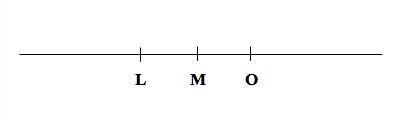
\includegraphics[scale=0.6]{unidimen.png}
\caption{Actors' ideal points in a unidimensional policy space}
\label{unidimen} 
\end{figure}
\\
% Actors' utility function
\indent Policy choice (\textit{x}) can be chosen from a proposal by L, (\textit{a}), a proposal by O, (\textit{b}), or a status quo policy (\textit{sq}. Formally, \textit{x} $\in$ \{\textit{a, b, sq}\}. All actors know the status quo policy, and it is the reversionary point in cases where the actors do not agree to pass a new law. Again, for simplicity and tractability, we assume that status quo policies are uniformly distributed throughout the unidimensional space. Each actor gets a maximum utility if a final policy outcome (\textit{x}) is equal to their ideal point (\textit{p} $\in$ \{\textit{l, m, o}\}). They have a single peak utility function such that the payoff is $-|p-x|$. The utility of all actors are given by
\\
$U_L = -|l-x|$\\
$U_M = -|m-x|$\\
$U_O = -|o-x|$
\\
% Actors' Strategies
\indent M is always given the legislative power to accept or reject a proposal. The median voter accepts a proposal if it gives a greater utility relative to the status quo and accepts an amendment if it gives greater utility than the previously proposed bills. Next, we consider L and O's strategies under several of the most common and most general types of legislative legislative powers: first proposal power, amendment power, second proposal power, and veto power. 

% First proposal power
\subsection{Strategies}
\subsubsection{First Proposal Power}
\indent Actors may have the right to propose any bill first. We model the actors' first proposal power by putting an actor on the top of a game tree and giving the actor the option of proposing and not proposing any legislation on some policy dimension. If the actor chooses to propose, the new bill has to be different from the status quo. Conceptually proposing first may mean having ex-ante veto power. That is to say, leaders are able to filter out proposals so that unwanted proposals can never be presented in a national assembly. This idea is similar to the concept of negative agenda-setting power \citep{coxmccubbins05}. On the other hand, proposing first may mean an exclusive right to propose a bill for certain policy areas. For example, bills related to national budget and taxations are required to be proposed exclusively by the executive in some dictatorships \citep{barkan09}. Such countries include Bangladesh, Bolivia, Ethiopia, Fiji, and Ghana \citep{ccpdata}. 
\subsubsection{Amendment Power}
\indent In proposing an amendment, the new proposal has to be different from the original proposal and the status quo. Amendment power is understudied in both the formal and empirical literature on the U.S. Congress (though, see \citet{monroeetal18}) and on legislative behavior more generally. Yet, as we show below, amendment power can be extremely beneficial, both as a means of making inroads into affecting policy as the opposition and as a means of protecting policy positions as the leader. Note that while amendment power is straightforwardly identified in most legislative bodies, it is sometimes shrouded in a more complex procedure (see, for example, \citet{roberts05} on the motion to recommit).
\subsubsection{Second Proposal Power}
\indent Note that this is distinct from amendment power; amendments, for our purposes, only occur when a proposal on some policy dimension has already been made, while second proposals occur on some policy dimension only when the other actor has passed on the opportunity to propose a new policy on that dimension. Thus, second proposals only compete (initially) against the status quo. If proposing, the new policy has to be different from the status quo. Many constitutions allow individual legislators to propose bills, but often with some constraints, such that proposals may only be offered after a leader first had a chance to submit a policy proposal for consideration \citet{barkan08}.   
\subsubsection{Veto Power}
\indent Here, we mean ex-post veto power; the ability to reject a final proposal at the end of the arrangement of legislative procedures. Veto power in this sense is perhaps the most commonly studied type of legislative power, especially in the U.S. context where this is the focal point of presidential legislative power \citep{krehbiel99, tsebelis02}. Note that this is distinct from and, as we show, not always redundant to the exercise of ex-ante veto power. Here, we do not consider the implications of the ability to override an ex-post veto but think this worthy of future study.
\\
% Actors' available action changes depending on a legislative process
\indent In the remainder of the paper, we aim to learn how optimal strategies and policy outcomes change as these four legislative procedures are arranged in various ways. Broadly, we organize this exercise into two sections:  the leader has first proposal power in the first section, and the opposition has this power in the second section. As readers will see, this dichotomy generates important variation in the effects of the opposition's ability to `poison' the process and the leader's ability to mitigate those effects with procedural antidotes.
\section{When the Leader Has First Proposal Power}
% What it means for the leader to have the first proposal power
\indent Leaders often have the power to propose first. Indeed, this may be the most common and most important legislative power available to leaders and, in the simplest settings, the most powerful. 
% we will derive Model equilibrium with the logic of a spatial model
%The simplest version of this model involves the leader as an only proposer, where no vote is required and the opposition has no ability to poison the process; here, the opposition is essentially an observer and the leader is a dictator without even a median voter to worry about. In this case, the equilibria policy will always be at \textit{l}, the leader's most preferred outcome. 
In the simplest version of the model, which originated with \citet{romerrosenthal78}, the leader has first proposal power and bills pass by majority voting in a national assembly. Figure \ref{lpm} shows the game tree.  
\begin{figure}[h]
  \centering
  \begin{minipage}[b]{0.3\textwidth}
    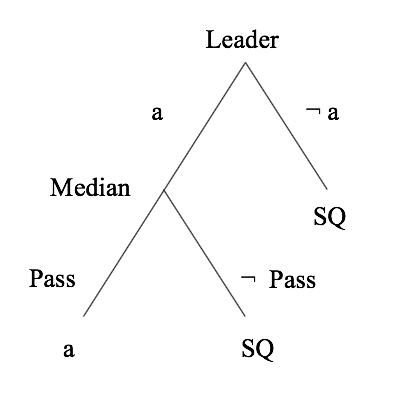
\includegraphics[width=\textwidth]{lpm}
    \caption{Leader's Exclusive Proposal Power paired with a Majority Voting}
    \label{lpm}
  \end{minipage}
  \hfill
  \begin{minipage}[b]{0.6\textwidth}
    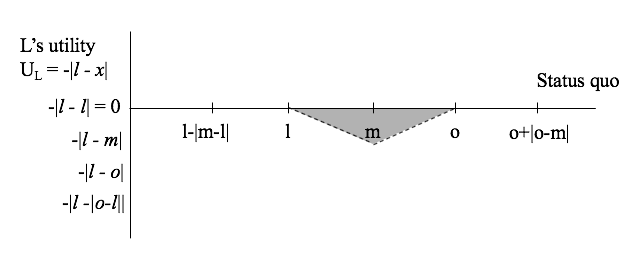
\includegraphics[width=\textwidth]{lpeq}
    \caption{L's total utility through status quos \newline from $l-2|m-l|$ to $o+2|o-m|$}
    \label{lpeq}
  \end{minipage}
\end{figure}
\FloatBarrier

%% How we derive the equilibrium
%\indent What are policy equilibria from Figure \ref{lpm}? To answer the question, we solve for the Subgame Perfect Nash Equilibrium. This requires that each actor's strategy be optimal, given the other actors' strategy after every possible history in the model \citep{osborne04}. In addition, actor's strategy should be optimal given the status quo. We assume status quos are uniformly distributed throughout the unidimensional space. That is, every status quo has an equal chance to be chosen by Nature at the beginning of the model. To clearly demonstrate how we solve the model, we analyze policy equilibria from six different status quos shown in Figure \ref{sq}. sq1 is located at $(l-\frac{1}{2}|m-l|)-(|m-l|)$, sq2 is located at $l-\frac{1}{2}|m-l|$, sq3 is located at $l+\frac{1}{2}|m-l|$, sq4 is located at $m+\frac{1}{2}|o-m|$, sq5 is located at $o+\frac{1}{2}|o-m|$, and sq6 is located at $(o+\frac{1}{2}|o-m|)+ (|o-m|)$.
%\\
%\begin{figure}[h]
%\centering
%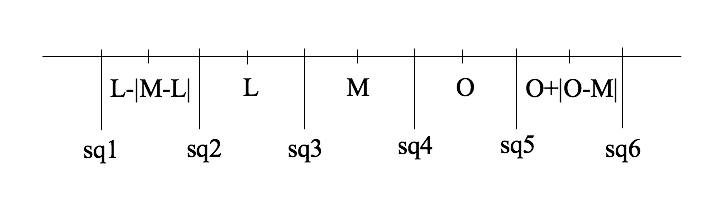
\includegraphics[scale=0.4]{sq.png}
%\caption{Status Quos in a Unidimensional Policy Space}
%\label{sq} 
%\end{figure}
%\\
%% Model play sq1
%\indent Imagine that Nature chooses sq1 which is located at the far left of L (i.e., $(l-\frac{1}{2}|m-l|)-(|m-l|)$). To maximize payoff, the leader would want to propose at $a=l$. After the leader's proposal, legislators' majority vote will decide whether or not they pass it. Therefore, the median voter's role becomes critical as it acts as a veto player. In this particular case, the median voter also gets a larger payoff with $a=l$ compared to the payoff with sq1. Therefore, the median voter will pass the proposal, and $a=l$ becomes the equilibrium policy. The policy loss for the leader is 0. The same equilibrium policy is produced with sq2 with the same logic of the game.
%\\
%% Model play sq3
%\indent If Nature chooses sq3 located between L and M, the leader cannot expect the median voter to pass any proposal that is less than sq3 (such as $a=l$) because it gives less payoff to the median voter compared to the payoff it will get with sq3. The leader would not propose anything that is greater than sq2 because the new bill will make the leader worse off. Therefore, sq3 stays as an equilibrium policy. The policy loss for the leader $-|l-sq3|$.
%\\
%% Model play sq4
%\indent If Nature chooses sq4 located between M and O, the leader can expect the median voter to pass a proposal as long as it makes the median voter better off or indifferent compared to having sq3. In fact, any bills that are between sq3 and $m-|sq3-m|$ are acceptable by the median voter. Among these bills, the leader can maximize its payoff by proposing $a=m-|sq3-m|$. the median voter will pass it and the equilibrium policy will be $a=m-|sq3-m|$. The policy loss for the leader $-|l-(m-|sq3-m|)|$.
%\\
%% Model play sq5
%\indent If Nature chooses sq5 located on the right side of O, the leader can maximize its payoff by proposing at $a=l$, and the median voter will pass it because $a=l$ gives a larger payoff than sq5. Therefore, $a=l$ will be the equilibrium policy. The policy loss for the leader is 0.
%\\
% Visualization of equilibria policies
\indent Figure \ref{lpeq} visualizes the leader's policy losses in this simplest version of the model. Throughout the rest of the paper, we use figures that operate identically. Thus, we think it useful to be somewhat deliberate in articulating the implications of different values within the figure at this first opportunity. 
\\
\indent The X-axis represents the status quo policy at each point on that dimension, and the Y-axis shows how far policy ends up from the leader's ideal point for each corresponding status quo on the X-axis (i.e., a leader's utility). Thus, the shaded area represents policy losses that the leader incurs for all status quos on dimension x. For example, Figure \ref{lpeq} shows that a leader incurs policy losses only when the status quo lies between $l$ and $o$. In particular, the loss is maximized when the status quo lies at $m$. When the status quo lies at $m$, the leader's utility is $-|l-m|$. When the policy outcome is $x=l$, it is exactly on the leader's most preferred policy and thus the dotted line intersects the x-axis at this point showing that the leader's utility is maximized for that status quo (and, in this case, all status quos to the left of that point). If $sq=o$  (and all those to the right of that point), then the leader incurs no policy loss because the new policy will be at $x=l$.
\\
% Preview of next subsection
\indent For the remainder of this section--and in a sense, for the remainder of the paper, we treat this model as our baseline. That is, this is a model where the leader acts like a sort of agenda-setting dictator; the opposition acts as a bystander here, with no agenda-setting weapons to challenge the leader with. In the next subsection, we examine what happens when a leader takes the `poison' of giving the opposition the right to amend a proposal and how leader's 'antidotes'--amendment power--work to counteract any policy loses that accrue. 

%We show that the overall policy losses increase due to this poison. We then introduce possible antidote procedures that the leader can institute: Leader's amendment power, Leader's veto power, and the combination of the amendment and veto power. We show that antidote procedures do not work effectively to reduce a significant amount of policy losses for a leader. However, we suggest that there is a possibility that the leader may still minimize policy losses while attaining benefits of sharing legislative power with the opposition if the leader knows that status quo is distributed around the leader.
\FloatBarrier
\subsection{Poison 1: Opposition's Amendment Power}
% Model
\indent Here, the opposition is given an institutional role and an option to amend bills proposed by a leader (game tree in Figure \ref{lpoam}). Figure \ref{lpoaeq} visualizes policy losses for a leader across all status quos. The policy loss is $-|l-m|$ in the status quo ranges left to $l-|m-l|$ and right to $m$. When the status quo lies between $l-|m-l|$ and $m$, the policy loss is less than $-|l-m|$ and it becomes 0 when the status quo lies at $l$. Notice that the leader's losses here are substantial; L faces policy losses if and only if the status quo lies between $l$ and $m$ in the baseline model (Figure \ref{lpeq}); however, L faces additional policy losses throughout all status quo ranges from $l-2|m-l|$ to $o+2|o-m|$ in Figure \ref{lpoaeq}.
\begin{figure}[h]
  \centering
  \begin{minipage}[b]{0.3\textwidth}
    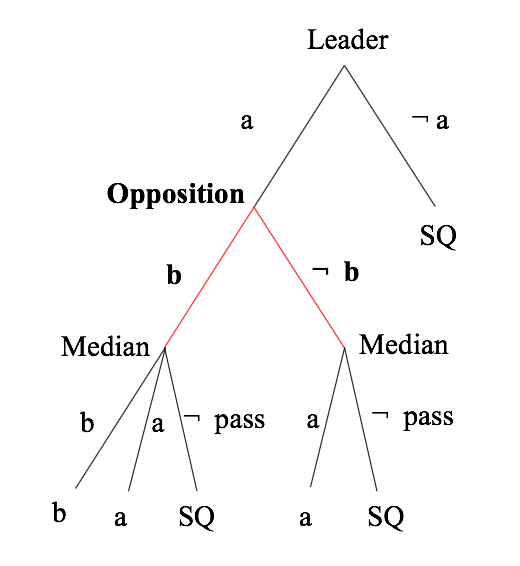
\includegraphics[width=\textwidth]{lpoam.png}
    \caption{Poison: Opposition's Amendment Power}
    \label{lpoam}
  \end{minipage}
  \hfill
  \begin{minipage}[b]{0.6\textwidth}
    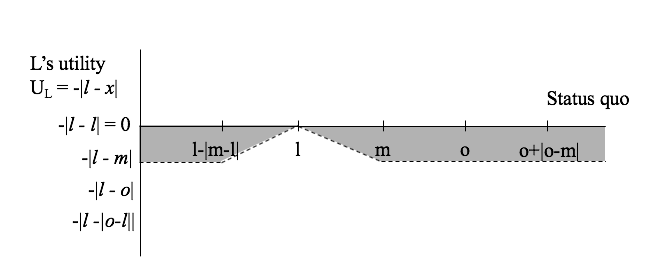
\includegraphics[width=\textwidth]{lpoaeq.png}
    \caption{L's total utility through status quos \newline from $l-2|m-l|$ to $o+2|o-m|$}
    \label{lpoaeq}
  \end{minipage}
\end{figure}
\FloatBarrier
%% Model play sq1 - possibility
%\indent As before, we run this spatial model to derive Subgame Perfect Nash Equilibrium with particular status quos in Figure \ref{sq}. If Nature chooses sq1 (i.e., $(l-\frac{1}{2}|m-l|)-(|m-l|)$), the leader would want to propose $a=l$ to minimize its policy loss. If the leader proposes at $a=l$, the opposition is now given a constitutional right to make a counteroffer to be voted on in a national assembly. The amendment by the opposition should be passed by the median voter. Given $a=l$, the median voter will pass any bill as long as it is between $a=l$ and $m+|m-l|$. Among these bills, the opposition maximizes by amending the bill at $b=m+|m-l|$. The median voter will pass it, and the leader does not have any other institutional procedure to invoke. In this case, the policy loss for the leader is $-|l-(m+|m-l|)|$. 
%\\
%% Model play sq1 - Optimal
%\indent However, it is not the leader's optimal strategy. The leader, in fact, can do better by proposing $a=m$. If the leader proposes $a=m$, the opposition cannot make an alternative amendment that will better satisfy the median voter. Therefore, the median voter will pass $a=m$, and the leader loses $-|l-m|$ when the status quo lies at sq1. 
%\\
%% Model play sq2
%\indent If the status quo lies at sq2, the leader may want to propose $a=l$, but the opposition will be able to amend it to its side by proposing a bill that will make the median voter slightly better off than $a=l$. Therefore, the opposition would propose at $b=o-\alpha$. $\alpha$ represents an infinitesimal number. The median voter would pass $b=o-\alpha$. Expecting this, the leader would not propose any bill and keep the status quo because $-|l-sq1|$ is less policy loss than $-|l-(o-\alpha)|$. Therefore, sq2 stays as a new bill and the leader incurs a policy loss of $-|l-sq1|$.
%\\
%% Model play sq3
%\indent If the status quo lies at sq3, the leader cannot make a proposal that simultaneously makes both the leader and the median voter better off. Therefore, the leader does not propose and sq3 stays. The leader incurs a policy loss of $-|l-sq3|$.
%\\
%% Model play sq4
%\indent If the status quo lies at sq4, the leader would move it to its side by proposing a bill that will make the median voter slightly better. That is, the leader could propose at $a=m-|sq4-m|-\alpha$. Then the opposition gets an option to amend it. The opposition would bring it back to its side by proposing $b=m+|sq4-m|-\alpha$. Instead, the leader can better by proposing $a=m$ because $-|l-m|>-|l-b|$. The opposition cannot amend the bill because the median voter already maximizes its utility with $a=m$. Therefore, $a=m$ becomes the equilibria policy and the leader incurs a policy loss of $-|l-m|$. sq5 and sq6 garner the same equilibrium.

% Antidote: leaders' amendment power
\indent Next, consider what happens if the leader institutes its own amendment power as an antidote to the poison of the opposition's amendment power (game tree in Figure \ref{lpoalam}). To model this, we allow the leader an option to make a counter-offer after the opposition makes an amendment to the bill proposed by the leader. If the leader makes an amendment ($a$) to the opposition's amendment ($b$), the median voter gets to pass either $a$ or $b$ or pass none. For simplicity, and without consequence, we assume that the median voter considers a most recent amendment first (that is, if the leader makes an amendment, $a$, it is voted first). This antidote turns out to be totally ineffective at counteracting the poison, as leader utility under this arrangement is identical to that shown in Figure \ref{lpoaeq}. Compared to the policy loss without the antidote (Figure \ref{lpoaeq}, we do not observe any difference in Figure \ref{lpoalameq}.
\begin{figure}[h]
  \centering
  \begin{minipage}[b]{0.3\textwidth}
    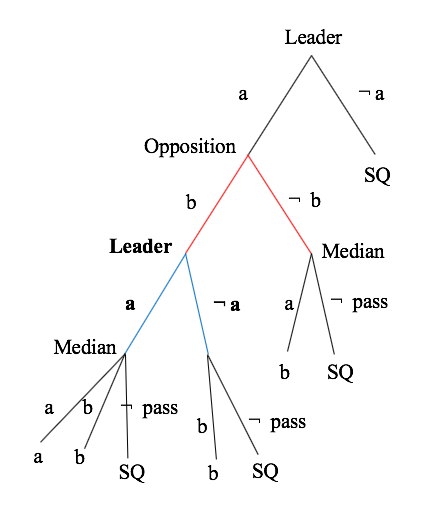
\includegraphics[width=\textwidth]{lpoalam.png}
    \caption{Leader's Amendment Power paired with Opposition's Amendment Power}
    \label{lpoalam}
  \end{minipage}
  \hfill
  \begin{minipage}[b]{0.6\textwidth}
    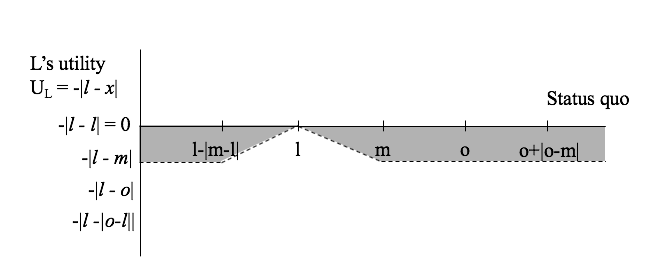
\includegraphics[width=\textwidth]{lpoalameq.png}
    \caption{L's total utility through status quos \newline from $l-2|m-l|$ to $o+2|o-m|$}
    \label{lpoalameq}
  \end{minipage}
\end{figure}
\FloatBarrier
%% Policy loss for a leader
%\indent To find out changes in policy losses with leader's amendment power, we find the Subgame Perfect Nash Equilibrium.  To demonstrate the gameplay, we use six possible status quos in Figure \ref{sq} again and elaborate the gameplay to find an equilibrium policy associated with each status quo.  
%\\
%% Model play sq1
%\indent Imagine that Nature chooses sq1 in Figure \ref{sq} as the status quo. The leader would want to bring it to $a=l$ to minimize its policy loss. If the leader proposes $a=l$, the opposition now has the option to make an amendment. The opposition can pass a new bill as long as the median voter feels indifferent compared to $a=l$. Since we assume equidistance between $|M-L|$ and $|O-M|$. The opposition can expect that the median voter will feel indifferent between $a=l$ and $b=o$, and so the opposition can propose $b=o$. But this time, the leader can also exercise the amendment power. The leader can make a counteroffer back to $a=l$. The median voter will pass $a=l$. 
%\\
%% Model play sq1 on the perspective of the opposition
%\indent However, $a=l$ is not an optimal outcome for the opposition. In fact, when the opposition gets to make an amendment, the opposition can amend the bill to $b=m$. The leader cannot make a further amendment because the median voter would not pass anything further than $b=m$. Therefore, the median voter passes $b=m$, and it becomes the equilibrium policy when the status quo is at sq1. For the opposition, $-|o-m|$ is a greater payoff than $-|o-l|$. For the median voter, the equilibrium is what it most prefers. For the leader, $-|l-m|$ is a greater payoff than $-|l-sq1|$. That is, the leader gets a greater payoff by proposing any bill than not proposing at all (keeping the status quo) even if the leader's proposal will be amended to $m$. Therefore, the equilibrium policy given sq1 is $m$. The leader loses $-|l-m|$. 
%\\
%% Model play sq2
%\indent If Nature chooses sq 2 in Figure \ref{sq}, the leader's optimal strategy is not to propose anything and keep the status quo as the equilibrium policy. If the leader proposes at $a=l$, the opposition will amend it to $b=m$. In this case, the leader cannot make a counteroffer that the median voter will pass. The equilibrium policy will be $b=m$, and the leader losses $-|l-m|$. It is a greater loss than $-|l-sq2|$, which is the payoff that the leader gets if the leader does not propose any. Therefore, the leader does not propose and sq2 stays as the equilibrium policy. The policy loss for the leader is  $-|l-m|$.
%\\
%% Model play sq3
%\indent If Nature chooses sq3 in Figure \ref{sq}, again, the leader's optimal strategy is not to propose anything and keep the status quo as the equilibrium policy. In this case, any proposal on the left side of sq3 will not be accepted by the median voter, and the leader would not propose anything on the right side of sq3. Therefore, sq3 stays as the equilibrium policy and the leader losses $-|l-sq3|$.
%\\
%% Model play sq4
%\indent If Nature chooses sq4 in Figure \ref{sq}, the leader would be tempted to propose $a=m-|sq4-m|$ since it will be closer to the leader's most preferred policy and the median voter would be indifferent between sq4 and o propose $a=m-|sq4-m|$. If the leader does so, the opposition has the option to make a counteroffer and would propose $b=m$. The leader cannot make another amendment since the median voter will reject anything other than $m$. Proposing is still an optimal strategy for the leader because the leader incurs the policy loss of $-|l-sq4|$ which is greater than $-|l-m|$. Therefore, $b=m$ is an equilibrium policy and the leader losses $-|l-m|$. The same play happens for sq5 and sq6. 
%\\
%% Policy loss visualization

%\\
%\begin{figure}[h]
%\centering
%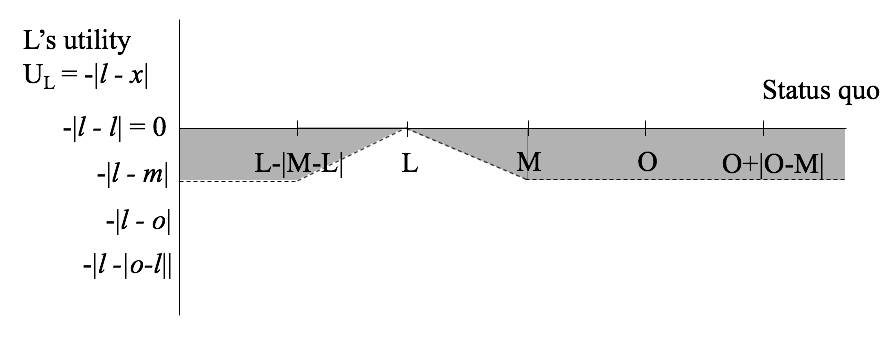
\includegraphics[scale=0.3]{lpoalaeq.png}
%\caption{Leader's Policy Losses from Model in Figure \ref{lpoalam}}
%\label{lpoalaeq} 
%\end{figure}
%\\
%\subsubsection{Antidote: Leader's Veto Power}

\indent Next, consider outcomes if we substitute the leader's counter-proposal power for an ex-post veto (game tree in Figure \ref{lpoalv}). To model this, we allow the leader an option to decide whether or not to assent a bill amended by the opposition and passed by the median voter. If the leader assents the bill, the opposition's amendment becomes a new law. If the leader does not assent to it (i.e., the leader vetos the bill), the status quo stays as a new law. Here again, the veto is an ineffective procedural antidote, as leader utility again tracks perfectly with that shown in Figure \ref{lpoaeq}. 
\begin{figure}[h]
  \centering
  \begin{minipage}[b]{0.3\textwidth}
    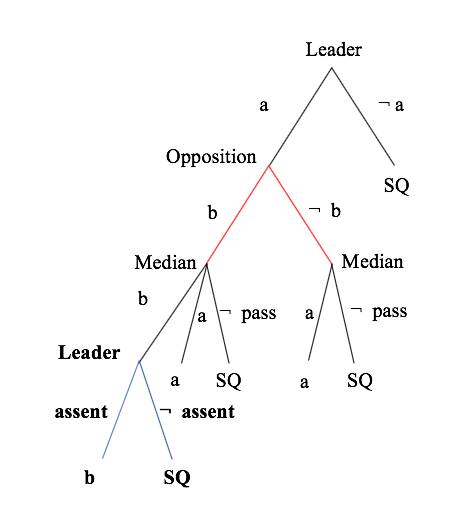
\includegraphics[width=\textwidth]{lpoalv.png}
    \caption{Leader's Veto Power paired with Opposition's Amendment Power}
    \label{lpoalv}
  \end{minipage}
  \hfill
  \begin{minipage}[b]{0.6\textwidth}
    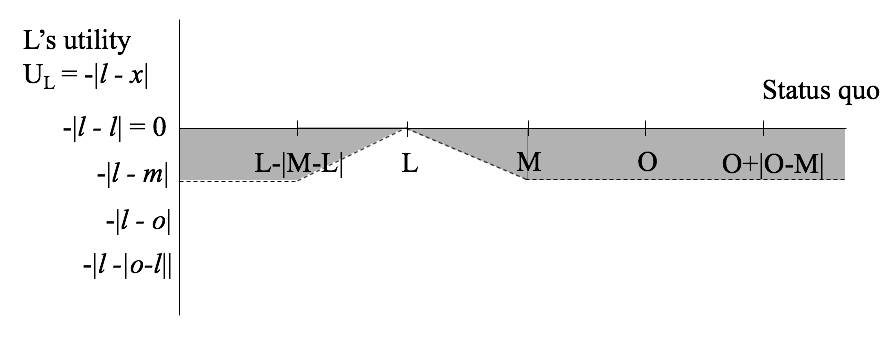
\includegraphics[width=\textwidth]{lpoalveq.png}
    \caption{L's total utility through status quos \newline from $l-2|m-l|$ to $o+2|o-m|$}
    \label{lpoalveq}
  \end{minipage}
\end{figure}
\FloatBarrier

%\indent We find the Subgame Perfect Nash Equilibrium to see any changes in policy losses for the leader. Again, we use six possible status quos in Figure \ref{sq} to demonstrate the gameplay.
%\\
%\indent If Nature chooses sq1 in Figure \ref{sq}, the leader would want to bring it to $a=l$ to minimize its policy losses. If the leader proposes $a=l$, the opposition has an option to amend it. The opposition would be better off to amend it to $b=o$ assuming that the median voter will pass $b=0$ as long as the median voter is indifferent between $a=l$ and $b=o$. Here the leader has the power to veto the bill, and the leader will veto it because $b=0$ makes the leader worse than $sq1$. The leader can do better than having $sq1$ if the leader proposes at $a=m$. $a=m$ is closer to the leader than $sq1$ while any amendment by the opposition will not pass by the median voter. Therefore, $x=m$ is the equilibrium policy if the status quo is $sq1$.
%\\
%\indent If Nature chooses sq2 in Figure \ref{sq}, the leader would want to bring it to $a=l$. The opposition now can amend it, but the opposition is aware of the executive's veto power. Therefore, the opposition will propose an amendment that will both maximize their payoffs among the bills that are acceptable to the leader. The leader would like to pass any bill that are between $sq2$ and $L+|L-sq2|$. Among these bills, the opposition will propose an amendment at $b=L+|L-sq1|$. The median voter passes and the leader assents it. The equilibrium policy is $x=L+|L-sq1|$ given the status quo is sq2.  
%\\
%\indent If Nature chooses sq3 in Figure \ref{sq}, the leader can expect the median voter to reject any proposal that is less than sq3. The leader does not propose any bill. Therefore, the equilibrium policy is sq3 given the status quo is sq3.
%\\
%\indent If Nature chooses sq4, the leader would want to propose $a=m-|sq4-m|$, a proposal that maximizes a leader's utility among proposals that are acceptable for the median voter. However, the leader can expect that the opposition can amend the bill back to $b=sq4$. %If we assume that the median voter and veto player will pass a bill that gives them the same utility as the status quo.
%The leader can do better by proposing $a=m$ so that the opposition cannot amend it further. $a=m$ also gives a greater utility for the leader than sq4. Therefore, the equilibrium policy is $a=m$ given the status quo is sq4. The same logic applies for sq5 and sq6.
%\\
%\begin{figure}[h]
%\centering
%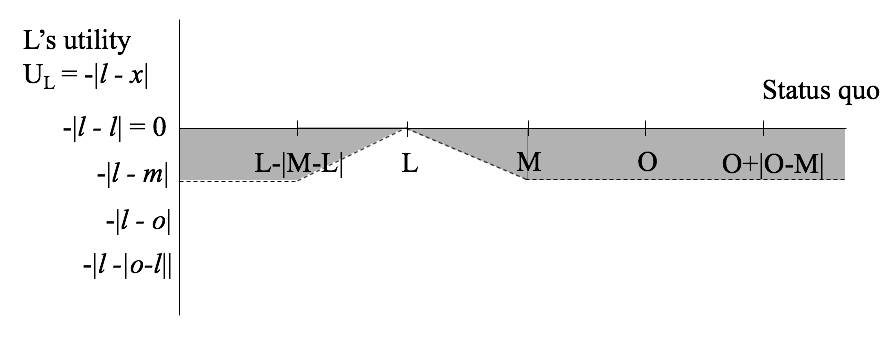
\includegraphics[scale=0.3]{lpoalveq.png}
%\caption{Leader's Policy Losses from Model in Figure \ref{lpoalv}}
%\label{lpoalveq} 
%\end{figure}
%\\
%\subsubsection{Antidotes: Leader's Amendment Power and Veto Power}
\indent Even when we consider both antidotes together (game tree in Figure \ref{lpoalalv}), losses remain the same. In short, opposition amendment power is a very damaging poison when the leader makes the first proposal, and the leader's available antidotes do little to inoculate the leader against policy losses in this case. In the next subsection, we examine a number of antidote procedures that can be used against second poison - Opposition's Second Proposal Power.
\begin{figure}[h]
  \centering
  \begin{minipage}[b]{0.3\textwidth}
    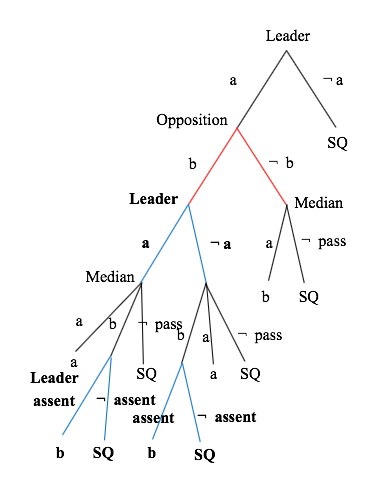
\includegraphics[width=\textwidth]{lpoalalv.png}
    \caption{Leader's Amendment Power and Veto Power paired with Opposition's Amendment Power}
    \label{lpoalalv}
  \end{minipage}
  \hfill
  \begin{minipage}[b]{0.6\textwidth}
    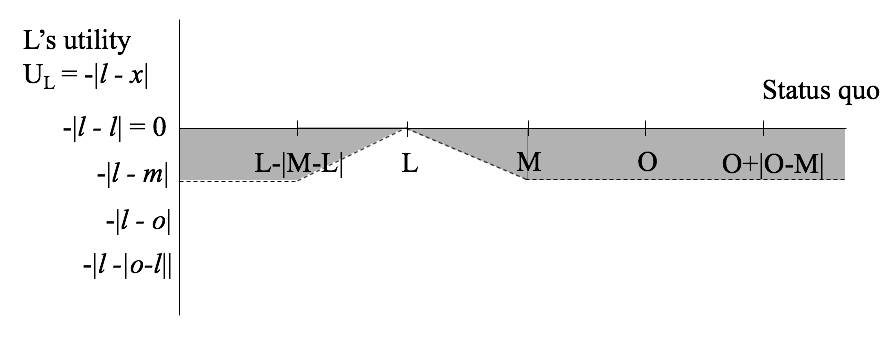
\includegraphics[width=\textwidth]{lpoalalveq.png}
    \caption{L's total utility through status quos \newline from $l-2|m-l|$ to $o+2|o-m|$}
    \label{lpoalalveq}
  \end{minipage}
\end{figure}
\FloatBarrier

%\indent We find the Subgame Perfect Nash Equilibrium to see any changes in policy losses for the leader. 
%\\
%\indent If Nature chooses sq1 in Figure \ref{sq}, the leader would want to bring it to $a=l$ to minimize its policy losses. The opposition can amend it to $b=o$ since the median voter will be indifferent between $a=l$ and $b=o$. However, the opposition can expect that the leader can amend the bill back to $a=l$ and also that the leader can veto $b=o$ even if it is passed by the median voter. Expecting this, the opposition would propose $b=m$ so that the leader cannot further amend it while it gives the leader a greater utility than having sq1. Therefore, the equilibrium policy is $x=m$ given the status quo is sq1.  
%\\
%\indent If Nature chooses sq2 in Figure \ref{sq}, the leader would want to minimize policy losses by proposing $a=l$. Then the opposition would amend it to $b=l+|l-sq2|$. The median voter passes it because it gives a greater utility than $a=l$. The leader would not veto it because the leader is indifferent between $sq1$ (the policy if the leader vetoes $b$) and $b=l+|l-sq2|$. Therefore, the equilibrium policy is $x=l+|l-sq2|$ given that status quo is sq2.
%\\
%\indent If Nature chooses sq3 in Figure \ref{sq}, the leader cannot make a proposal that makes both the leader and the median voter better off. Therefore, the leader does not propose a bill or any proposal that is less than sq3 will be rejected by the median voter. Therefore, the equilibrium policy is sq3 given that the status quo is sq3.
%\\
%\indent If Nature chooses sq4 in Figure \ref{sq}, the leader may want to propose $a=m-|sq4-m|$. Then the opposition can amend it back to $b=m+|sq4-m|$ which is sq4. But the opposition knows that the leader can amend it again back to $a=m-|sq4-m|$, and the median voter would pass. The opposition would get a greater utility by proposing $b=m$ than letting $a=m-|sq4-m|$ become a new policy. Therefore, the equilibrium policy is $x=m$ given the status quo is sq4. The same logic applies for sq5 and sq6.
%\\
%\indent Figure \ref{lpoalalveq} visualizes the leader's policy losses across possible status quos given the legislative process in Figure \ref{lpoalalv}.
%\begin{figure}[h]
%\centering
%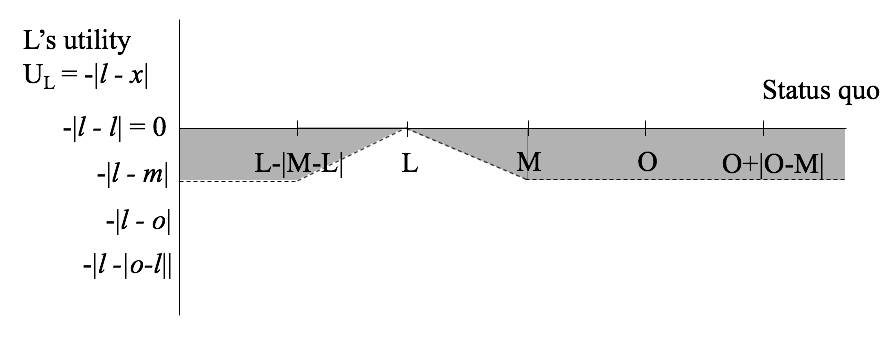
\includegraphics[scale=0.3]{lpoalalveq.png}
%\caption{Leader's Policy Losses from Model in Figure \ref{lpoalalv}}
%\label{lpoalalveq} 
%\end{figure}
%\\
\FloatBarrier
\subsection{Poison 2: Opposition's Second Proposal Power}
\indent The opposition may have the power to propose a bill only after being given the opportunity by the leader; we refer to this as second proposal power. To model this, we give the opposition an institutional option to propose a bill if the leader decides not to propose any bills or fails to pass a new bill (game tree in Figure \ref{lpos}). As before we find the Subgame Perfect Nash Equilibrium for this arrangement of legislative procedures and subsequent versions where the leader employs various antidotes. 
\begin{figure}[h]
  \centering
  \begin{minipage}[b]{0.3\textwidth}
    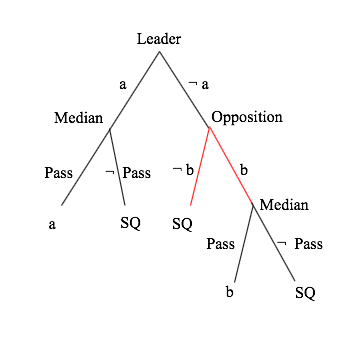
\includegraphics[width=\textwidth]{lpos.png}
    \caption{Poison 2: Opposition's Second Proposal Power}
    \label{lpos}
  \end{minipage}
  \hfill
  \begin{minipage}[b]{0.6\textwidth}
    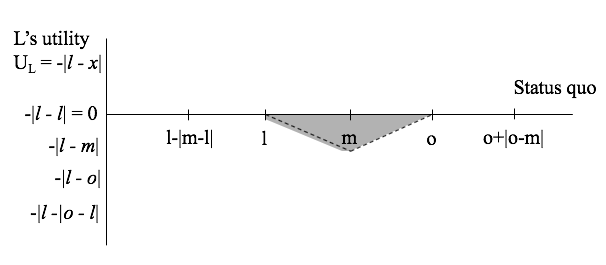
\includegraphics[width=\textwidth]{lposeq.png}
    \caption{L's total utility through status quos \newline from $l-2|m-l|$ to $o+2|o-m|$}
    \label{lposeq}
  \end{minipage}
\end{figure}
\FloatBarrier

%\indent If Nature chooses sq1 in Figure \ref{sq}, the leader would want to maximize utility by proposing $a=l$. The median voter will pass it since $-|m-l|>-|m-sq1|$. The opposition does not have an institutional role here since the leader proposed something. Therefore, the equilibrium policy is $x=l$ when the status quo is sq1. The logic is the same for sq2 as well. The equilibrium policy given sq2 is $x=l$.
%\\
%\indent If Nature chooses sq3 in Figure \ref{sq}, the leader cannot find a proposal that will increase utility for both the leader and the median voter as the status quo is in between them. In the legislative process where the leader proposes and the median voter votes (in Figure \ref{lpm}), the leader does not propose anything and the equilibrium policy is $x=sq3$. However, not proposing is not an optimal strategy for the leader in the legislative process in Figure \ref{lpos}. What is different in Figure \ref{lpos} is that the opposition now has the power to propose a bill to be voted by the median voter if the leader does not propose any bill. If the leader does not propose a bill when the status quo is sq3, the opposition would propose a bill, $b=m+|m-sq3|$, since it is the bill that incurs the greatest utility for the opposition among the bills ($[sq3,|m+m-sq3|]$) that the median voter prefers to sq3. However, the leader now incurs the policy loss of $-|(m+|m-sq3|)-l|$. The leader can reduce policy losses by proposing $a=sq+\alpha$. Again $\alpha$ represents a positive infinitesimal number. What is happening is that the leader compromises a proposal little by $\alpha$ so that the median voter accepts the bill. By doing this, the leader reduces policy losses from $-|(m+|m-sq3|)-l|$ to $-|(sq3+\alpha)-l|$. Therefore, the equilibrium policy is $x=sq3+\alpha$ when the status quo is sq3.
%\\
%\indent If Nature chooses sq4 in Figure \ref{sq}, the leader would want to minimized policy losses by proposing $a=m-|sq4-m|$ because it gives the leader the greatest utility among bills that are acceptable for the median voter (i.e., [$m-|sq4-m|, sq4$]). Therefore, the equilibrium policy is $x=m-|sq4-m|$ when the status quo is sq4.
%\\
%\indent If Nature chooses sq5 in Figure \ref{sq}, the leader would want to minimize policy losses by proposing $a=l$. The median voter accepts it because $a=l$ gives a greater utility than $sq5$. Since the leader proposed, the opposition does not have an institutional role to take further actions. Therefore, the equilibrium policy is $x=l$ when the status quo is sq5. The same logic applies to sq6. Therefore, the equilibrium policy is $x=l$ when the status quo is sq6. 
\indent Figure \ref{lposeq} visualizes the leader's policy losses across all possible status quos given the arrangement of procedural poison and antidote in Figure \ref{lpos}. Strikingly, this poison is much less damaging to the leader's policy utility than opposition amendment power. Here, policy loss for the leader only slightly exceeds the baseline case where the opposition has no legislative power at all, and this small policy loss is by the leader's own hand as a preventative measure. In the baseline model, for status quo's between $l$ and $m$, the leader will not make a proposal because no policy move will increase her utility but also satisfy $m$ relative to the status quo. Here, if the leader employs that strategy, the opposition will take advantage of making a proposal after the leader passes the opportunity to do so. This strategy of no proposal moves policy as far to the right as possible, between $m$ and $o$. To avoid this relatively larger policy loss, the leader will make a proposal $\alpha$ to the right of the current status quo, thus eliminating the oppositions ability to make a second proposal.

%\subsubsection{Antidote: Leader's Amendment Power}
\indent As a first antidote, we give the leader the power to propose a counter-offer to the opposition's amendment. We model this antidote by allowing the leader the option to propose a counter-offer if the opposition proposes a bill after the leader decides not to propose first (game tree in Figure \ref{lposla}). Here, again, the antidote is ineffective at mitigating the (admittedly small) policy losses that accrue to the leader from the opposition's second proposal poison; the equilibria policies are the same as the no-antidote condition shown in Figure \ref{lposeq}. 
\begin{figure}[h]
  \centering
  \begin{minipage}[b]{0.3\textwidth}
    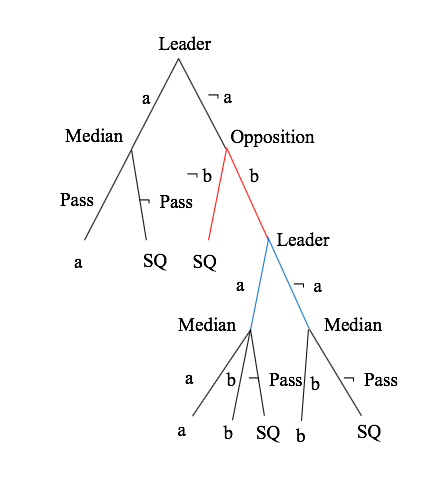
\includegraphics[width=\textwidth]{lposla.png}
    \caption{Leader's Amendment Power paired with Opposition's Second Proposal Power}
    \label{lposla}
  \end{minipage}
  \hfill
  \begin{minipage}[b]{0.6\textwidth}
    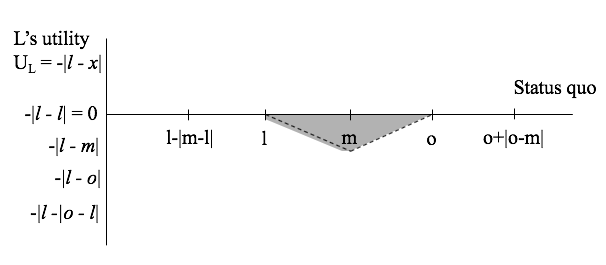
\includegraphics[width=\textwidth]{lposlaeq.png}
    \caption{L's total utility through status quos \newline from $l-2|m-l|$ to $o+2|o-m|$}
    \label{lposlaeq}
  \end{minipage}
\end{figure}
\FloatBarrier
\indent One interesting observation in this iteration of the model is that invoking the antidote procedure to amend a bill proposed by the opposition is not an optimal strategy for the leader when the status quo is between $l$ and $m$. When the status quo is in this interval, as in the baseline model, the `winset' is null as the leader cannot find a proposal that will simultaneously make better off both the leader and the median voter.\footnote{The `winset' is a set of policies (excluding the status quo) that are preferred by both the leader and the median voter. For a formal definition, see \citet{tsebelis02}.} If the leader does not offer a new policy and lets the opposition propose, the opposition will propose $b=m$ knowing that the leader cannot amend $b$, as the median will prefer $b$ to any amendment. In this case, the leader is better off to propose $a=sq+\alpha$ at the beginning of the process because it is closer to the leader than $b=m$. Once $a=sq+\alpha$ is offered by the leader, the opposition does not have an institutional role to counteract the passage. 
\\
\indent This oddity goes away when we instead consider the effect of giving the leader's ex-post veto power as an antidote to the opposition's second proposal power (game tree in Figure \ref{lposlv}). Here, the veto eliminates the very small policy losses created by the opposition's second proposal power (Figure \ref{lposlveq}; equilibrium policy losses match those under the baseline model that is shown in Figure \ref{lpeq}. Similarly, when we combine both antidotes, giving the leader both amendment and veto power in response to the oppositions second proposal power (game tree in Figure \ref{lposlalv}), policy losses are identical to the no-antidote condition (Figure \ref{lposlalveq}). The veto is doing the work, however, while the amendment power is essentially irrelevant as an antidote.

\begin{figure}[h]
  \centering
  \begin{minipage}[b]{0.3\textwidth}
    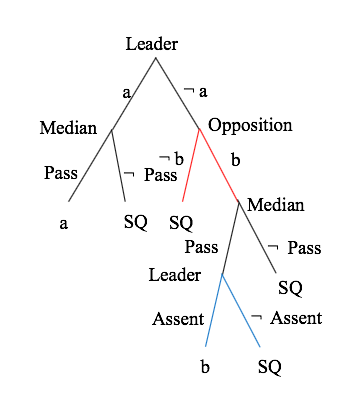
\includegraphics[width=\textwidth]{lposlv.png}
    \caption{Leader's Veto Power paired with Opposition's Second Proposal Power}
    \label{lposlv}
  \end{minipage}
  \hfill
  \begin{minipage}[b]{0.6\textwidth}
    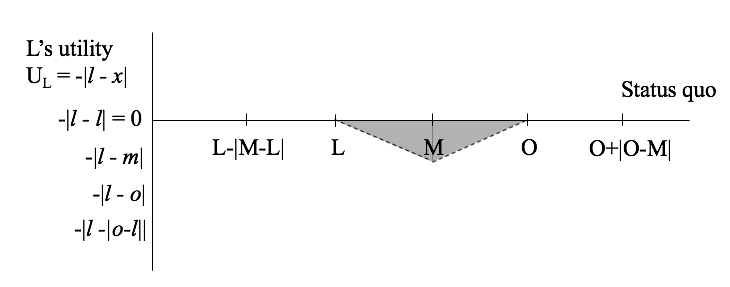
\includegraphics[width=\textwidth]{lposlveq.png}
    \caption{L's total utility through status quos \newline from $l-2|m-l|$ to $o+2|o-m|$}
    \label{lposlveq}
  \end{minipage}
\end{figure}
\FloatBarrier

\begin{figure}[h]
  \centering
  \begin{minipage}[b]{0.3\textwidth}
    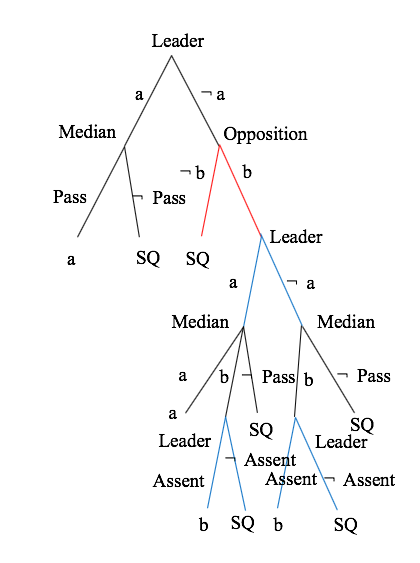
\includegraphics[width=\textwidth]{lposlalv.png}
    \caption{Leader's Amendment power and Veto Power paired with Opposition's Second Proposal Power}
    \label{lposlalv}
  \end{minipage}
  \hfill
  \begin{minipage}[b]{0.6\textwidth}
    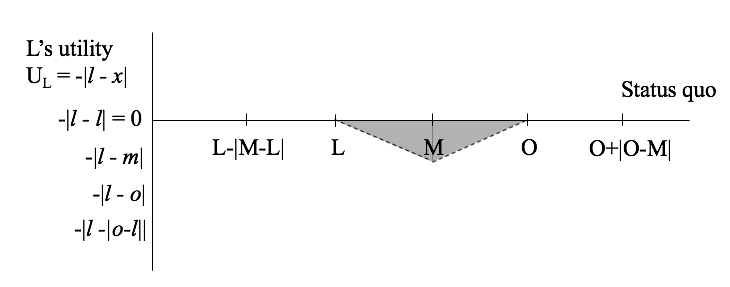
\includegraphics[width=\textwidth]{lposlalveq.png}
    \caption{L's total utility through status quos \newline from $l-2|m-l|$ to $o+2|o-m|$}
    \label{lposlalveq}
  \end{minipage}
\end{figure}
\FloatBarrier

\indent Before moving on to the next section, where we consider the final--and most potent--poison, it will be useful to take some inventory of the points so far. When the leader has first proposal power, her policy utility suffers significantly larger deficits when the opposition has the power to amend the leader's proposals than when the opposition can offer a ``second'' proposal after the leader passes. Moreover, neither of the proposed procedural antidotes--separately or in combination--reduced opposition amendment-driven policy losses, whereas even the very small policy losses suffered by the leader at the hands of opposition second-proposal power were mitigated by the leader's veto power. Thus, if the leader has the first proposal power, she will almost surely pick the second-proposal poison if given the option.\footnote{\citet{woodissert} shows that this is empirically the case in dictatorships, and leaders in dictatorships often pair the opposition's second proposal power with the leader's veto power.}
%for this result . The results are the same with the model without an antidote procedure except when the status quo is $sq3$. Compared to the result from the model with an antidote (i.e., $x=sq3+\alpha$), the leader reduces the policy loss by $\alpha$.\footnote{\cite{woodissert} points out that equilibrium policies are the same between the `dictatorial process' in Figure \ref{lpm} and more `democractic process' in Figure \ref{lposlv}. \cite{woodissert} suggests that leaders in authoritarian states may manage policy losses by changing legislative processes from Figure \ref{lpm} to Figure \ref{lposlv} when they have to share some legislative power with the opposition.} When the status quo is $sq3$, it is optimal for the leader to invoke the veto power. When the leader does not propose a bill, the opposition proposes a bill (given the assumption about the benefits of proposing, $\beta$). Given the location of the opposition's policy position, the opposition would not propose a bill less than $sq3$, but the proposal greater than $sq3$ will be vetoed by the leader. Then the $sq3$ remains as the new policy.\footnote{the result is the same without the assumption of the benefit of proposing. Without this assumption, the opposition also does not propose anything, and $sq3$ remains as the new policy.}  
%\\
%\begin{figure}[h]
%\centering
%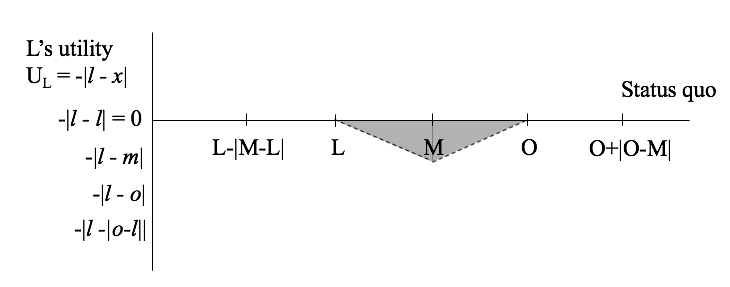
\includegraphics[scale=0.4]{lposlveq.png}
%\caption{Leader's Policy Losses from Model in Figure \ref{lposlv}}
%\label{lposlveq} 
%\end{figure}
%\\
%\subsubsection{Antidote: Leader's Amendment Power and Veto Power}
%\indent Figure \ref{lposlveq} shows the equilibria of the case where the leader has both the amendment power and veto power. The results are the same with the model without an antidote procedure except when the status quo is $sq3$. Compared to the result from the model with an antidote (i.e., $x=sq3+\alpha$), the leader reduces the policy loss by $\alpha$. One thing to note is that, when the status quo is $sq3$, it is not optimal for the leader to invoke the amendment power, but it is optimal to use the veto power. If the leader chooses to propose a bill, the best the leader can do is $x=sq3+\alpha$. If the leader does not proposes a bill and lets the opposition do so, the leader can veto whatever the opposition proposes. It renders the status quo to stay as a new policy. If the opposition expects the leader to amend the opposition's proposal, it is possible that the opposition will propose $b=m$ so that the leader cannot amend the proposal. Instead of amending it, the leader will let it pass by the median voter and veto, thereby rendering $sq3$ to be the new policy. 
%\\
%\begin{figure}[h]
%\centering
%\includegraphics[scale=0.4]{lposlvlaeq.png}
%\caption{Leader's Policy Losses from Model in Figure \ref{lposlvlaeq}}
%\label{lposlveq} 
%\end{figure}
%\\
%\FloatBarrier
\section{When the Opposition Has First Proposal Power}
\indent In this section, we consider our final procedural poison: opposition first proposal power. We set it apart as its own section for two reasons. First, giving the opposition first proposal power changes the structure of the game such that the possible poison-antidote combinations deviate slightly from the previous section. Second, baseline policy losses for this condition are substantially larger, and thus we consider deviations from a different baseline (which we explain below).  
\\
\indent To model the opposition's first proposal power, we let the opposition have the option to propose $b$ or not propose anything. If the opposition proposes $b$, the median voter decides whether or not to pass it. Figure \ref{opm} shows the arrangement of legislative procedures under this condition. 

\begin{figure}[h]
  \centering
  \begin{minipage}[b]{0.3\textwidth}
    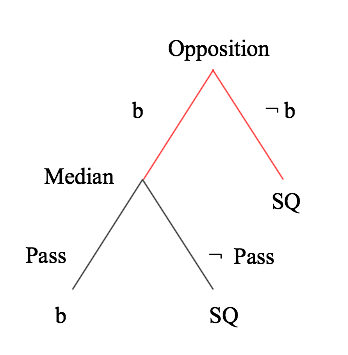
\includegraphics[width=\textwidth]{opm.png}
    \caption{Opposition's First Proposal Power}
    \label{opm}
  \end{minipage}
  \hfill
  \begin{minipage}[b]{0.6\textwidth}
    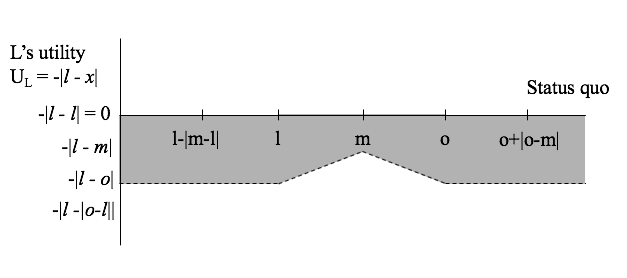
\includegraphics[width=\textwidth]{opmeq.png}
    \caption{L's total utility through status quos from \newline $l-2|m-l|$ to $o+2|o-m|$}
    \label{opmeq}
  \end{minipage}
\end{figure}
\FloatBarrier

%\indent When the status quo is at, the opposition propose at $b=o$ to maximize its utility, and the median voter passes it because $b=o$ gives a greater utility than $sq1$. Therefore, the equilibrium policy when the status is $sq1$. The same is true for $sq2$. 
%\\
%\indent If Nature chooses $sq3$, $b=o$ is no longer preferred by the median voter. The median voter will pass a bill as long as the bill is between [$sq3$, $m+|m-sq3|$]. Among bills in this range, the opposition maximizes its utility by proposing $m+|m-sq3|$. Therefore, the equilibria policy is $b= m+|m-sq3|$  when status quo is $sq3$.
% \\
% \indent If Nature chooses $sq4$, the opposition does not find a proposal that will simultaneously make both the median voter and the opposition better. Anything left of $sq4$ will make the opposition worse off while anything right of $sq4$ will make the median voter worse off. Since the opposition gets positive utility from proposing a bill. it makes a proposal (that is right of $sq4$) and the median voter will not pass it. Therefore, the equilibrium policy is $sq4$ when the status quo is $sq4$. 
% \\
% \indent If nature chooses $sq5$, the opposition proposes $b=o$ to maximize utility, and the median voter will pass it because $b=o$ gives a greater utility than $sq5$. Therefore, the equilibrium policy is $b=o$ when the status quo is $sq5$. The same is true for $sq6$.
% \\
 \indent Figure \ref{opmeq} shows the leader's policy losses for all possible status quos. Given that the leader plays only an observer's roll in this baseline model, comparisons to losses under the first two poisons have an apples-to-oranges quality to them. With that in mind, we note that policy losses for the leader are dramatically larger in this condition. Here, the leader's \textit{smallest} policy loss $-|l-m|$ (where the status quo is at $m$), which is her \textit{largest} loss from the previous two poisons. As we move through our antidotes in the remainder of the section, however, a more striking apples-to-apples comparison will emerge: the leader's policy losses only drop back below this level with certain antidotes, and even then only for limited intervals of status quos.

\subsection{Antidote: Leader's Second Proposal Power}
\indent For our first antidote, we consider outcomes when the leader has the option to propose (i.e. make a second proposal) if the opposition does not propose any bill or if that bill fails passage by M (game tree in Figure \ref{opls}). As Figure \ref{oplseq} shows, leader's policy losses under this condition are only slightly mitigated here. The logic is identical to that which \textit{caused} slight leader losses when the opposition had second proposal power: the opposition will move policy away from their ideal point by $\alpha$ for all status quos between $m$ and $o$ to avoid much larger moves away from his ideal point by way of a leader's second-proposal. 
\begin{figure}[h]
  \centering
  \begin{minipage}[b]{0.3\textwidth}
    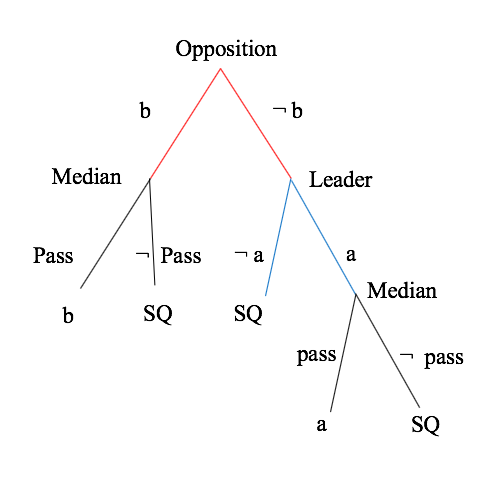
\includegraphics[width=\textwidth]{opls.png}
    \caption{Leader's Second Proposal Power paired with Opposition's First Proposal Power}
    \label{opls}
  \end{minipage}
  \hfill
  \begin{minipage}[b]{0.6\textwidth}
    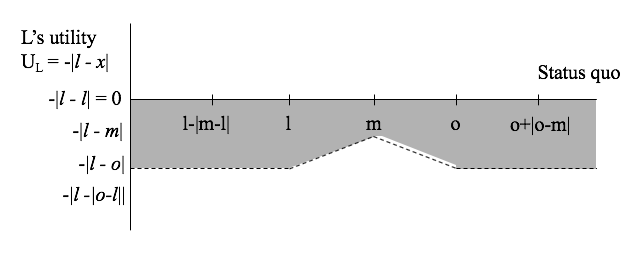
\includegraphics[width=\textwidth]{oplseq.png}
    \caption{L's total utility through status quos from \newline $l-2|m-l|$ to $o+2|o-m|$}
    \label{oplseq}
  \end{minipage}
\end{figure}
\FloatBarrier
%\indent Figure \ref{oplseq} shows leader's policy losses throughout all status quo when the leader institutes leader's second proposal power. Policy losses are not too different from the legislative process without the leader's second proposal power (Figure \ref{opmeq}). What is different is that when status quo is around $sq4$, the opposition would not let the leader propose even when the opposition cannot find a proposal that will simultaneously make both the opposition and the median voter better. If the opposition lets the leader propose a bill, the leader will propose $a=m-|sq4-m|-\alpha$ to make the median voter prefer $a$ to $sq4$. Consequently, the leader reduces $\alpha$ much of policy loss when the status quo is $sq4$.

\subsection{Antidote: Leader's Amendment Power}
\indent When the leader's amendment power is the antidote (game tree in Figure \ref{opla}), however, policy losses change considerably. As we see in Figure \ref{oplaeq}, compared to the leader's losses under the no-antidote condition (shown as the area between the X-axis and the dotted line), the leader's policy losses are significantly smaller. Over much of the range (all status quos to the left of $m$ and to the right of $o+|o-m|$), a policy now moves to $m$, cutting the leader's losses by half in many cases. 
% We model the leader's amendment power by giving the leader option to propose a counteroffer after the opposition proposes a bill, $b$. If leader makes an amendment, $a$, the median voter will either pass one of $a$ and $b$ or reject them both, thereby making the status quo the new bill. Figure \ref{opla} shows the legislative process.
\begin{figure}[h]
  \centering
  \begin{minipage}[b]{0.3\textwidth}
    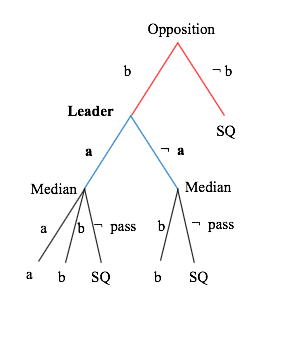
\includegraphics[width=\textwidth]{opla.png}
    \caption{Leader's Amendment Power paired with Opposition's First Proposal Power}
    \label{opla}
  \end{minipage}
  \hfill
  \begin{minipage}[b]{0.6\textwidth}
    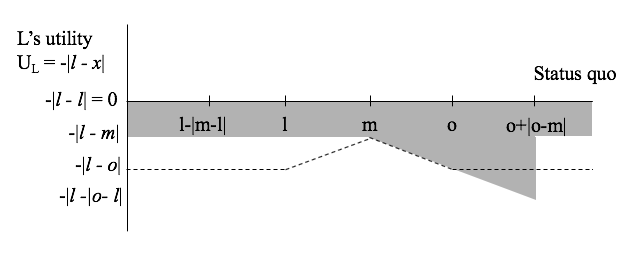
\includegraphics[width=\textwidth]{oplaeq.png}
    \caption{L's total utility through status quos from \newline $l-2|m-l|$ to $o+2|o-m|$}
    \label{oplaeq}
  \end{minipage}
\end{figure}
\FloatBarrier

\indent The amendment antidote is not beneficial for all status quos though. The leader suffers larger policy loses \textit{because of} her amendment power for status quos between $o$ and $o+|o-m|$. Here, the optimal strategy for the opposition is not to propose a new policy, whereas, in the no-antidote condition, the opposition moved these status quos to $o$. The opposition foresees that the leader will amend any proposal that the opposition makes to some point between $l$ and $m$, making the opposition worse off than they are under the status quo. To avoid this, they forgo the move left for all of these status quos which, perversely, would be better for all three actors in the game. 

\subsection{Antidote: Leader's Veto Power}
\indent Next, we model an arrangement where the leader is able to exercise the ex-post veto power as an antidote to the opposition's first proposal power (game tree in Figure \ref{oplv}). Figure \ref{oplveq} shows the equilibrium policies for all status quos under this arrangement. Here, the opposition can maximize utility by proposing $b=o$ as long as the leader prefers $b=o$ to the status quo. This includes all status quos left of $l-|o-l|$ and right of $o$. For all status quos between $l-|o-l|$ and $l$, the opposition will move policy as far to the right as the leader will allow (i.e. prefer the new policy to the status quo). All status quos between $l$ and $o$ will remain unchanged.    
\begin{figure}[h]
  \centering
  \begin{minipage}[b]{0.3\textwidth}
    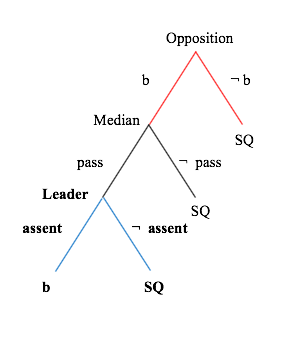
\includegraphics[width=\textwidth]{oplv.png}
    \caption{Leader's Veto Power paired with Opposition's First Proposal Power}
    \label{oplv}
  \end{minipage}
  \hfill
  \begin{minipage}[b]{0.6\textwidth}
    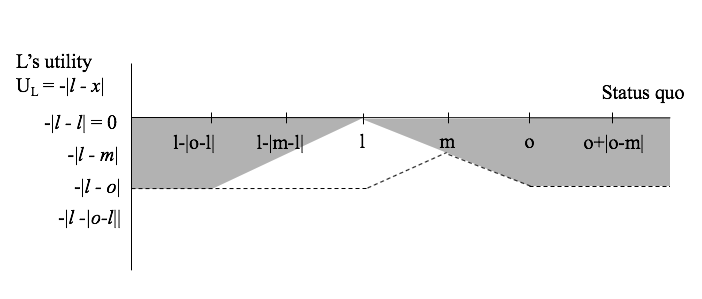
\includegraphics[width=\textwidth]{oplveq.png}
    \caption{L's total utility through status quos from \newline $l-2|m-l|$ to $o+2|o-m|$}
    \label{oplveq}
  \end{minipage}
\end{figure}
\FloatBarrier

\indent While both amendment and veto power significantly reduce leader's losses, comparing Figures \ref{oplaeq} and \ref{oplveq} highlights important differences in \textit{which} status quos are better protected be each antidote. For more extreme status quos (consider those to the left of $l-|m-l|$ and to the right of $o+|o-m|$), leader's losses are cut in half with the amendment antidote relative to the veto antidote or the baseline (depicted in Figure \ref{savedbyamend} by darker areas). Yet, for status quos in the middle of the space surrounding $l$, the veto causes losses to fall toward zero the closer they are to the leader's ideal point. Thus, while our primary aim in this paper is to consider policy losses across the entire space, there is a lesson here for future work: poisons and antidotes may be strategically chosen to fit the particular status quo distribution of legislative policy environment.

\begin{figure}[h]
\centering
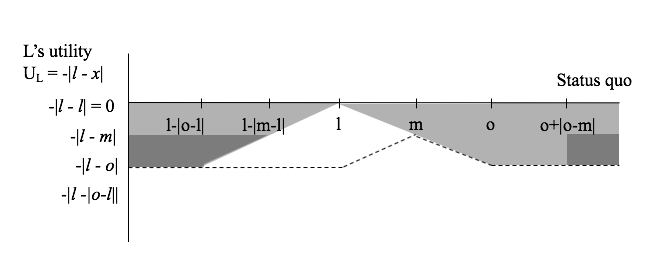
\includegraphics[scale=0.4]{savedbyamend.png}
\caption{Policy Loss Reduced by L's Amendment Antidote}
\label{savedbyamend} 
\end{figure}
\FloatBarrier


\subsection{Antidotes: Pair-Wise Combinations} %TODO Nate to fill the section
%\subsection{Antidote: Leader's Second Proposal Power and Amendment Power}
%\indent Now we examine the legislative process where the leader can amend bills proposed by the opposition while the leader also has the second proposal power. Figure \ref{oplals} shows the game tree that maps actors' all possible actions in this legislative process.
%\\
\begin{figure}[h]
  \centering
  \begin{minipage}[b]{0.3\textwidth}
    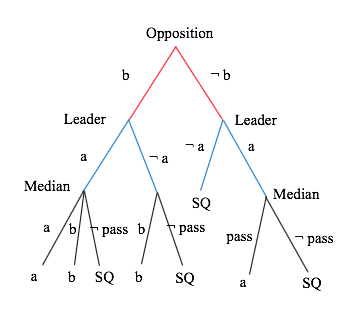
\includegraphics[width=\textwidth]{oplals.png}
    \caption{Leader's Second Proposal and Amendment Power Power paired with Opposition's First Proposal Power}
    \label{oplals}
  \end{minipage}
  \hfill
  \begin{minipage}[b]{0.6\textwidth}
    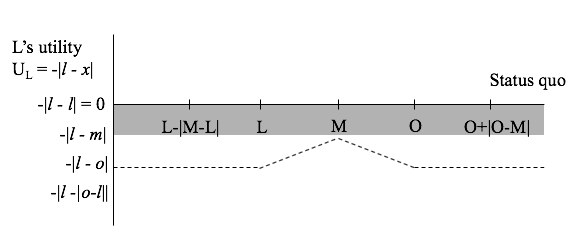
\includegraphics[width=\textwidth]{oplalseq.png}
    \caption{L's total utility through status quos from \newline $l-2|m-l|$ to $o+2|o-m|$}
    \label{oplalseq}
  \end{minipage}
\end{figure}
\FloatBarrier
%\indent Figure \ref{oplalseq} shows the equilibrium policies throughout all status quos in this legislative process. It is notable to see the final policy is $x=m$ in all status quo. In this legislative process, the leader has the power to propose a bill in both cases-when the opposition proposes a bill and when the opposition does not propose a bill. Without any of leader's antidote procedures, the opposition was able to legislate $x=o$ as long as the median voter preferred $x=o$ to status quos. For example, without leader's antidote procedures, if the nature chooses $sq1$, the opposition proposes $x=o$, and the median voter would pass it. With the leader's amendment power, however, the opposition can expect that the leader will amend the bill by proposing the counteroffer of $a=l-\alpha$. The amendment will be preferred by the median voter because it gives $\alpha$ much of more utility than $b=o$. In this case, the opposition gets $-|o-(l-\alpha)|$. If the opposition does not propose any thing, the leader now has the second proposal power and can maximize its utility by proposing $a=l$. The median voter will pass $a$ as it gives more utility than having $sq1$. In this case, the opposition gets $-|o-l|$. Both outcomes are not ideal for the opposition, as the opposition can decide to propose $b=m$, which gives greater utility for the opposition. By proposing $b=m$, it blocks the leader from proposing an amendment that the median voter would prefer. The same logic applies to all status quos.
%\\
%\subsection{Antidote: Leader's Second Proposal Power and Veto Power}
%\indent We examine how the leader can manage policy losses if the leader institutes its second proposal and veto power. Figure \ref{oplslv} shows the game tree that maps actors' all possible strategies under the legislative process. To model the leader's veto power, we allow the leader to decide whether it will assent or not assent the opposition's proposal, $b$, after the median voter passes it. The leader gets to propose $a$ under two cases: 1) if the median voter does not pass the opposition's proposal and 2) if the opposition does not propose a bill. If the leader gets to propose $a$, the median voter decides whether or not it will pass $a$.
%\\
\begin{figure}[h]
  \centering
  \begin{minipage}[b]{0.3\textwidth}
    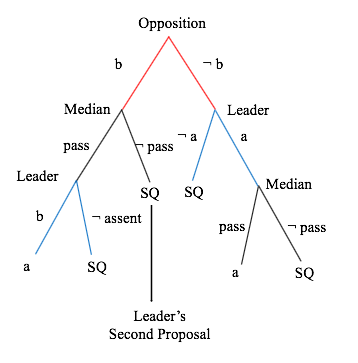
\includegraphics[width=\textwidth]{oplslv.png}
    \caption{Leader's Second Proposal Power and Veto Power paired with Opposition's First Proposal Power}
    \label{oplslv}
  \end{minipage}
  \hfill
  \begin{minipage}[b]{0.6\textwidth}
    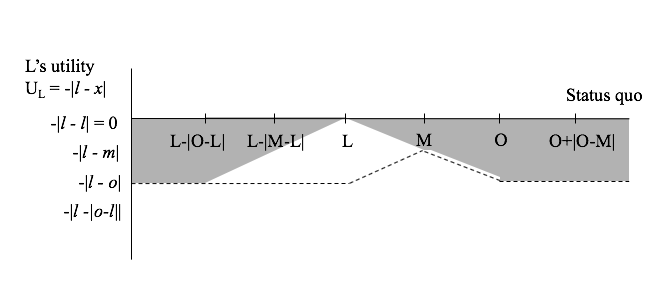
\includegraphics[width=\textwidth]{oplslveq.png}
    \caption{L's total utility through status quos from \newline $l-2|m-l|$ to $o+2|o-m|$}
    \label{oplslveq}
  \end{minipage}
\end{figure}
\FloatBarrier

%\indent Figure \ref{oplslveq} shows the equilibrium policies throughout all status quo for this legislative process. The result is similar to the legislative process where the leader pairs its veto power with the opposition's second proposal power (Figure \ref{oplveq}). The opposition now has to look for a bill that simultaneously make both the opposition and the leader better off. The difference is that the leader reduces a bit of ($\alpha$ much exactly) policy losses when the status quo is $sq4$. If Nature chooses $sq4$, the opposition cannot find a proposal that will simultaneously make both the opposition and the median voter better off. In a legislative process where the leader does not have the second proposal power, the opposition could simply keep the policy at the status quo by not proposing. In this legislative process, if the opposition does not propose, the leader would propose $a=(m-|sq4-m|)-\alpha$ to make the new policy closer to the leader, and the median voter would pass it. To prevent the leader from proposing anything, the opposition can propose $b=sq4-\alpha$ so that the median voter prefers $b$ to the status quo. That is to say, the second proposal power is not showing much marginal effect in reducing policy losses when used as an antidote procedure with the veto power.
%\\
%\subsection{Antidote: Leader's Amendment Power and Veto Power}
%\indent Now we examine policy losses from a legislative process where the leader institutes its amendment power and veto power while the opposition is the first proposer. Figure \ref{oplalv} shows the game tree that maps actors' all possible strategies. 

\begin{figure}[h]
  \centering
  \begin{minipage}[b]{0.3\textwidth}
    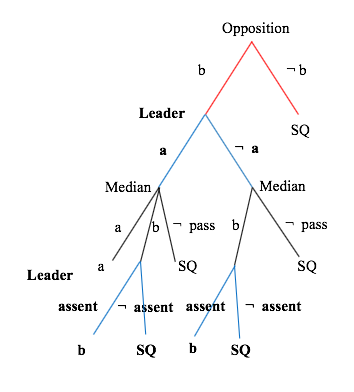
\includegraphics[width=\textwidth]{oplalv.png}
    \caption{Leader's Amendment Power and Veto Power paired with Opposition's First Proposal Power}
    \label{oplalv}
  \end{minipage}
  \hfill
  \begin{minipage}[b]{0.6\textwidth}
    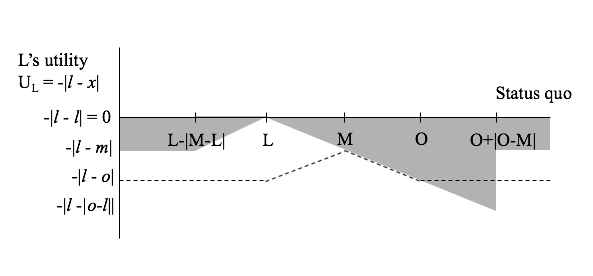
\includegraphics[width=\textwidth]{oplalveq.png}
    \caption{L's total utility through status quos from \newline $l-2|m-l|$ to $o+2|o-m|$}
    \label{oplalveq}
  \end{minipage}
\end{figure}
\FloatBarrier
%\\
%\indent Figure \ref{oplalveq} shows the equilibrium policies throughout all status quo. Similar to Figure \ref{oplaeq}, the leader's amendment power induces $x=m$ for $sq1$ and $sq6$. The veto power induces $x=l+sq$ for $sq2$. If Nature chooses $sq3$ and $sq4$, the leader is able to veto any attempt of the opposition to bring a new policy closer to $o$, thereby maintaining the status quos. The leader incurs more policy losses (compared to the legislative process without antidote procedures) because the opposition chooses rather not to propose anything for two reasons: 1) the opposition does not want the leader to make an amendment and 2) $x=m$ incurs more policy loss than $sq5$.
%\\
\subsection{Antidote: Leader's Second Proposal Power, Amendment Power, and  Veto Power}
\indent Finally, we consider the effect of all three antidote procedures in combination (game tree in Figure \ref{oplslalv}). As we see in Figure \ref{oplslalveq}\, and as one might expect, this arrangement of procedures is the Pareto dominant option; for all status quos in the space, leader losses are less than equal to or (in most cases) losses under any of the antidotes on their own. This combination performs especially well for status quos that lie near the leader's ideal point. 
\\
\indent Note, however, that when we take a broader view, this poison-antidote arrangement is still relatively bad for the leader. To see this, compare Figure \ref{oplslalveq} to Figure \ref{lpoaeq}, which shows policy losses for the leader when the leader has first proposal power and the opposition has the ability to amend. Recall that this was the worst case scenario for the leader across the first two poisons that we considered. The two figures are identical as shown in Figure \ref{}. In other words, the worst case scenario when the leader retains the ability to propose first is equivalent to the best case scenario when the leader concedes that institutional power to the opposition.\footnote{\citet{hartogmonroe11} incorporate this insight into their model of ``Costly Consideration.''}
\begin{figure}[h]
  \centering
  \begin{minipage}[b]{0.3\textwidth}
    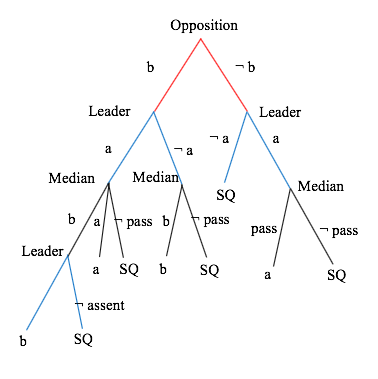
\includegraphics[width=\textwidth]{oplslalv.png}
    \caption{Leader's Second Proposal Power, Amendment Power and Veto Power paired with Opposition's First Proposal Power}
    \label{oplslalv}
  \end{minipage}
  \hfill
  \begin{minipage}[b]{0.6\textwidth}
    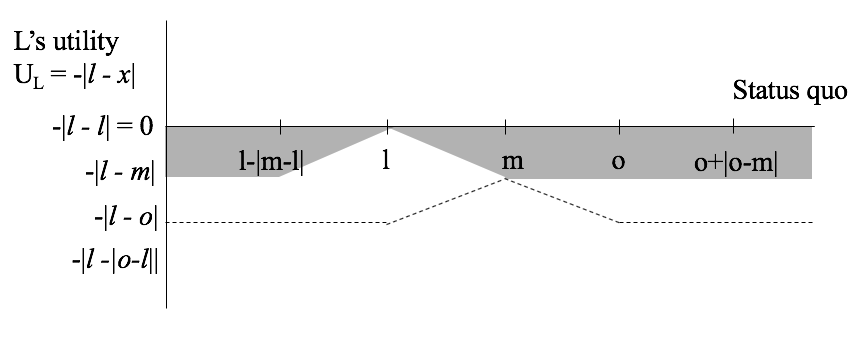
\includegraphics[width=\textwidth]{oplslalveq.png}
    \caption{L's total utility through status quos from \newline $l-2|m-l|$ to $o+2|o-m|$}
    \label{oplslalveq}
  \end{minipage}
\end{figure}
\FloatBarrier

%\indent Figure \ref{oplslalveq} shows the equilibrium policies throughout the status quos. Compared to other legislative processes elaborated above, this legislative process minimizes (when taken as a whole) the leader's policy losses. If Nature chooses $sq1$, $x=m$ as the opposition proposes $b=m$ to prevent the leader from amending it. With $sq2$ and $sq3$, the leader can keep the status quo with its veto power. If Nature choose $sq4$, the opposition again proposes $b=m$ so that the leader can neither amend it nor exercise the second proposal right. $x=m$ continues to be equilibrium policies for $sq5$ and $sq6$.

\section{Speculation on Which Poison is Preferable}
\indent Within the formal modeling exercise, our aim has been to focus entirely on the policy payoffs to the leader. Accordingly, our narrative to this point has offered comparisons of various institutional  based entirely on their relative maximizations of leader payoffs across a uniform distribution of status quos. In this section, we (informally) speculate about how leader preferences over institutions might change if we modify two assumptions: the shape of the status quo distribution and the "audience" value of particular institutions. 
\\
\indent First, as is common in much of the formal literature on legislative process, we work within a uniform status quo distribution. Yet, if we instead consider that many leaders will face status quo distributions with concentrations of status quos at certain points, some institutional arrangements will seem more appealing to the leader even if she only considers policy payoffs. 
\\
\indent For example, all of our preceding scenarios that include a leader first proposal or veto are increasingly advantageous for status quo distributions that are densely centered on the leader's ideal point, since she suffers very little policy loss for status quos near her ideal point under those institutional arrangements. Alternatively, when status quos are relatively extreme (i.e. left of the leader and right of the opposition), the leader should either prioritize first proposal power or implement a full compliment of antidotes in response to the oppositions first proposal power. Woo (2019) systematically defines and test these implications in her investigation of dictatorial regimes.
\\
\indent Second, to this point we have assumed that the value of institutions are simply a function of the resulting policy outcomes. Yet, we opened the paper noting that leaders may be compelled to share power. Thus, one might naturally wonder \textit{why} the leader is compelled to share power and how she can best satisfy the audience for that power sharing.
\\
\indent One approach to answering that question considers whether the "audience" is internal or external to the legislature. That is, if the audience for the sharing is the opposition themselves, then institutions that maximize the oppositions utility will be most valuable; here, opposition first proposal power may be preferred. On the other hand, if the audience is external, then giving the opposition a very visible set of procedural prerogatives--even if they amount to little policy advantage--may be most beneficial. 

\section{Conclusion}
\indent In this paper, we have used an analogy--poisons and antidotes--to further our understanding of the effects of pairing various agenda-setting institutions. In particular, we were motivated to understand the strategic institutional context in which leaders choose \textit{which} specific powers to share and to retain when they have an incentive or an obligation to share at least some legislative power with their opposition. This might occur in democracies when public opinion demands ``fairness'' or adherence to ``democratic'' norms; or it might occur in authoritarian regimes when leaders need to secure domestic allies or opponents or signal to international audiences.
\\ 
\indent Substantively, our models show that when the leader has first proposal power, her policy utility suffers significantly larger deficits when the opposition has the power to amend than when the opposition can offer a ``second'' proposal after the leader passes. Moreover, neither of the proposed agenda-setting antidotes that we considered (leader amendment or veto power)--separately or in combination--reduced opposition-amendment driven policy losses. Thus, when the leader has first proposal power, she will almost surely pick the second-proposal poison if given the option. 
\\
\indent Yet, perhaps the key point came in understanding the relative effect of leader versus opposition first proposal power. The worst case scenario when the leader retains the ability to propose first is equivalent to the best case scenario when the leader concedes that institutional power to the opposition. However, if a leader is forced to give up first proposal power, a combination of all three antidotes--amendment power, second proposal power, and veto power--can significantly mitigate her policy losses.
\\
\indent While our primary aim in this paper was to consider policy losses across the entire space, one possible lesson here for future work considers the implications of relaxing the uniform status quos distributional assumption. Poisons and antidotes--and particular combinations of the two--performed very differently across the range of status quos. Thus, leaders may have an incentive to strategically choose their mix of institutional concessions and protections to fit the particular status quo distribution of their legislative policy environment. The specifics of this strategic calculation would be fertile ground for future work.
\\
\indent More broadly, while abstract, we think the theoretical results in this paper have direct empirical applications. Most directly, our results suggest that some legislative institutional arrangements should be more likely than others, given the incentives of leaders to maximize policy utility. Relatedly, when we do observe variation in the combination of agenda powers modeled here, our results offer some guidance as to who the policy winners and losers should be and how big those wins and losses should be. While there has been some investigation of this in the domestic context (see \citet{carsonetal11} for example), there is much more to do in the comparative arena, especially in authoritarian legislatures.

%\section*{Acknowledgements} 



\bibliography{WooRef}
\bibliographystyle{apsr}

%\section*{Biographical Statement} 
%
%Ae sil Woo is a PhD Candidate in Political Science at the University of California, Merced, CA 95326. 
%\bigskip
%
%\noindent Nathan W. Monroe is an Associate Professor of Political Science at the University of California, Merced, CA 95326. 


\end{document} 